\documentclass[9pt, apectratio=43,unicode]{beamer}
\usetheme{Moscow}

\usepackage[utf8]{inputenc}
\usepackage[T2A]{fontenc}
\usepackage[main=russian,english]{babel}

\usepackage{amsmath,amssymb}

\renewcommand{\thefootnote}{\fnsymbol{footnote}}
\hypersetup{pdfauthor={Paul Ostanin}}

%\usepackage{concmath}
%\usepackage{euler}

\usepackage{mathtools}

\graphicspath{ {images/} }

\title[Моделирование земной ионосферы]{Динамическое моделирование земной ионосферы}
\author[Останин П. А.]{Останин Павел Антонович \\ \vspace{1ex} Выпускная квалификационная работа\\ \vspace{1ex} Научный руководитель: Кулямин Дмитрий Вячеславович}
\date{}

\newcommand{\colorhref}[2]{\href{#1}{\textcolor{miptbase!30!black}{#2}}}

\begin{document}

\begin{frame}[plain]
\titlepage
\end{frame}

\def\L{\mathcal{L}}

\section{Постановка задачи}
\subsection{Уравнение неразрывности}
\begin{frame}\frametitle{Постановка задачи}

Уравнение, описывающее эволюцию ионной концентрации: $$\dfrac{\partial n_i}{\partial t} = -div(n_i \vec{u}_\parallel)-div\left(n_i\dfrac{1}{B^2}[\vec{E}\times \vec{B}] \right)+$$ $$+div\left(D\left[\nabla_\parallel n_i +n_i\dfrac{1}{T_p}\nabla_\parallel T_p - \dfrac{n_i m_i}{2kT_p}\vec{g}_\parallel\right]\right)+[P-k_in_i]$$

Используемые приближения:
\begin{itemize}
\item[•] Динамическое преобладание амбиполярной диффузии;
\item[•] Одноионная постановка, квазинейтральность плазмы;
\item[•] Дипольное магнитное поле Земли;
\item[•] Приближение совпадения географических и магнитных полюсов;
\end{itemize}
\end{frame}


\subsection{Входящие в уравнение параметры}
\begin{frame}\frametitle{Входящие в уравнение параметры}
Для функций $P$, $k$, температур и концентраций $N_2$, $O_2$ и $O$ используются аналитические формулы: 
\begin{itemize}
\item[•] $T(z)=T_\infty - (T_\infty-T_0)\exp\left(-\dfrac{g}{RT_\infty}(z-z_0)\right),$ 

$T_{n\infty}=800$~К, $T_{i\infty}=950$~К, $T_{e\infty}=2200$~К.

\smallskip

\item[•] Для концентраций~---~Больцмановское распределение: $n_{O_2, N_2, O} (z)= n_{O_2, N_2, O} (z_0)\cdot \exp\left(-\dfrac{M_{O_2, N_2, O}g}{R_0T_n}(z-z_0)\right).$ 

На высоте $100$~км $n_{O_2} = 5{,}6\cdot 10^9$~см$^{-3}$, $n_{O} = 2{,}8\cdot 10^{10}$~см$^{-3}$, $n_{N_2} = 5{,}2\cdot 10^{10}$~см$^{-3}$.

\smallskip


\item[•] В дневное время $P=4\cdot10^{-7}n_O(z)$;

$k=1{,}2\cdot10^{-12}n_{N_2}(z)+2{,}1\cdot10^{-11}n_{O_2}(z)$
\end{itemize}
\end{frame}


\subsection{Метод расщепления, три постановки}
\begin{frame}\frametitle{Метод расщепления, три постановки}

Первое приближение: диффузия вдоль оси $z$:
$$\dfrac{\partial n}{\partial t} = P-kn+\dfrac{\partial}{\partial z}\left(D\dfrac{\partial n}{\partial z} + \left(\dfrac{1}{T_p}\dfrac{\partial T_p}{\partial z}+\dfrac{1}{H}\right) n\right)$$

Следующий шаг~---~учёт широтной зависимости: замена $D$ на $D\sin^2I$ ($I \approx \arctg(2\tg \varphi)$):
$$\dfrac{\partial n}{\partial t} =P-kn+\dfrac{\partial}{\partial z}\left[D\sin^2I\left(\dfrac{\partial n}{\partial z} + \left(\dfrac{1}{T_p}\dfrac{\partial T_p}{\partial z}+\dfrac{1}{H}\right) n\right)\right]$$

Более точный учёт широтной зависимости: $z$-диффузия в проекции (со смешанной производной):
$$\dfrac{\partial n}{\partial t} =P-kn+\dfrac{\partial}{\partial z}\biggl[D\sin^2 I\left(\dfrac{\partial n}{\partial z}+\left(\dfrac{1}{T_p}\dfrac{\partial T_p}{\partial z}+\dfrac{1}{H}\right)n\right)-$$ $$-\dfrac{1}{a}D\sin I\cos I\left(\dfrac{\partial n}{\partial\varphi}+\dfrac{1}{T_p}\dfrac{\partial T_p}{\partial\varphi}n\right)\biggr]$$ 

\end{frame}


\section{Численное моделирование}
\subsection{Требования к схемам и свойства решения}
\begin{frame}\frametitle{Требования к схемам и свойства решения}

\begin{itemize}
\item[•] Концентрация неотрицательна, для сохранения этого свойства используем монотонные схемы;
\item[•] Уравнение имеет закон сохранения массы, схемы должны быть консервативны;
\item[•] При постоянных $P$ и $k$ уравнение имеет стационарное решение;
\item[•] Характерные времена на нижней и верхней границах отличаются на несколько порядков, по времени используем неявные схемы.
\end{itemize}

\end{frame}


\subsection{Используемые схемы}
\begin{frame}\frametitle{Используемые схемы}
Для аппроксимации диффузионного слагаемого используется схема $$\dfrac{\partial}{\partial z}D\dfrac{\partial n}{\partial z} \approx \dfrac{1}{h_{i+1/2}}\left(\dfrac{D_{i+1/2}(n_{i+1}-n_i)}{h_i}-\dfrac{D_{i-1/2}(n_{i}-n_{i-1})}{h_{i-1}}\right)$$

Для одномерного уравнения исследованы следующие схемы:

\begin{itemize}
\item[•] В схеме $1$ потоковый член и граничное условие аппроксимируются с помощью направленных разностей; 
\item[•] В схеме $2$ потоковый член аппроксимируется центральной разностью, граничное условие~---~направленной разностью;
\item[•] Схема $3$ имеет согласованные граничное условие и схему, записанные с помощью центральных разностей.
\end{itemize}

Для уравнения со смешанной производной вводится $$u_\varphi=-\dfrac{1}{a}D\sin I \cos I\dfrac{1}{n}\dfrac{\partial n}{\partial \varphi}$$~---~нелинейная добавка добавка к эффективной скорости.

\end{frame}


\section{Результаты численных экспериментов}
\subsection{Воспроизведение дневного вертикального профиля электронной концентрации}
\begin{frame}\frametitle{Воспроизведение дневного вертикального профиля электронной концентрации}

\begin{figure}[H]
\center{
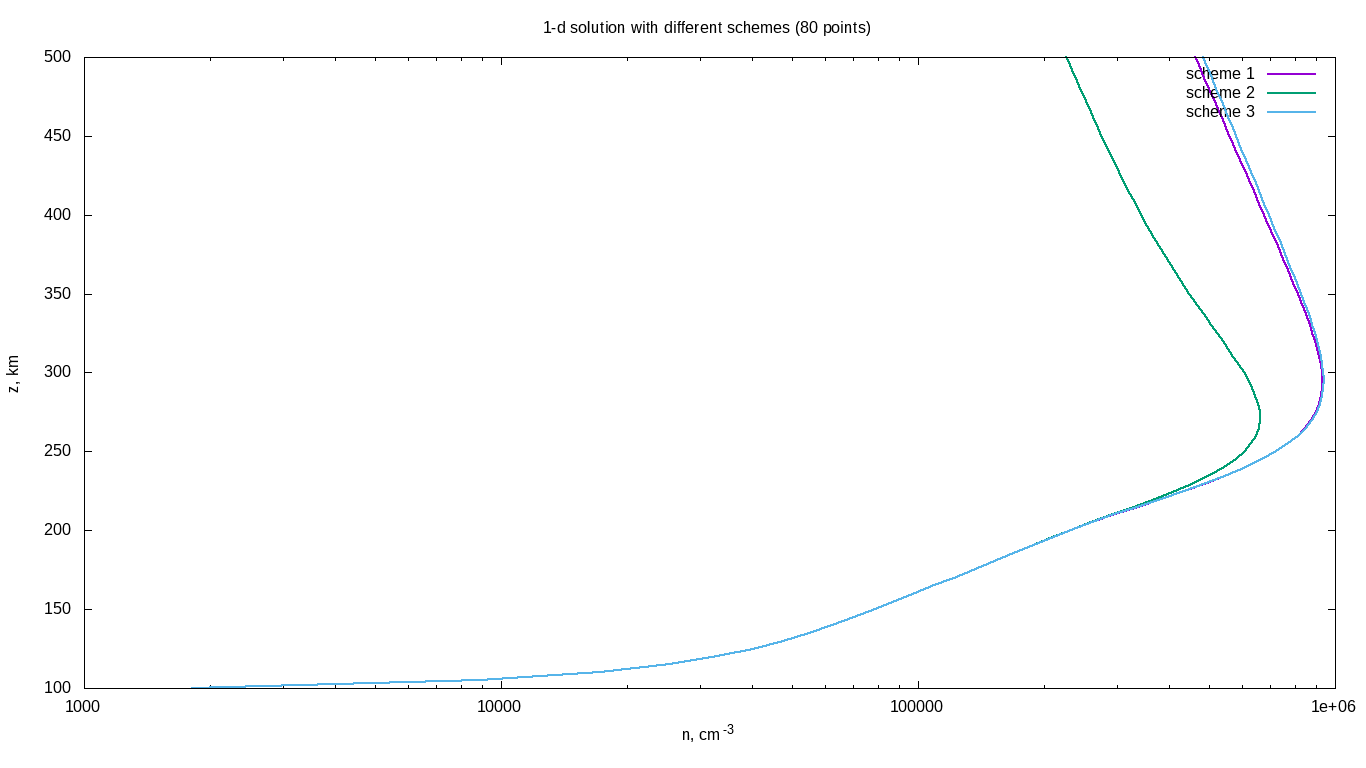
\includegraphics[scale=0.33]{1d_stationary_logscale_80}}
\caption{Стационарные решения на $80$ расчётных узлах.}
\end{figure}


\end{frame}

\begin{frame}\frametitle{Воспроизведение дневного вертикального профиля электронной концентрации}

\begin{figure}[H]
\center{
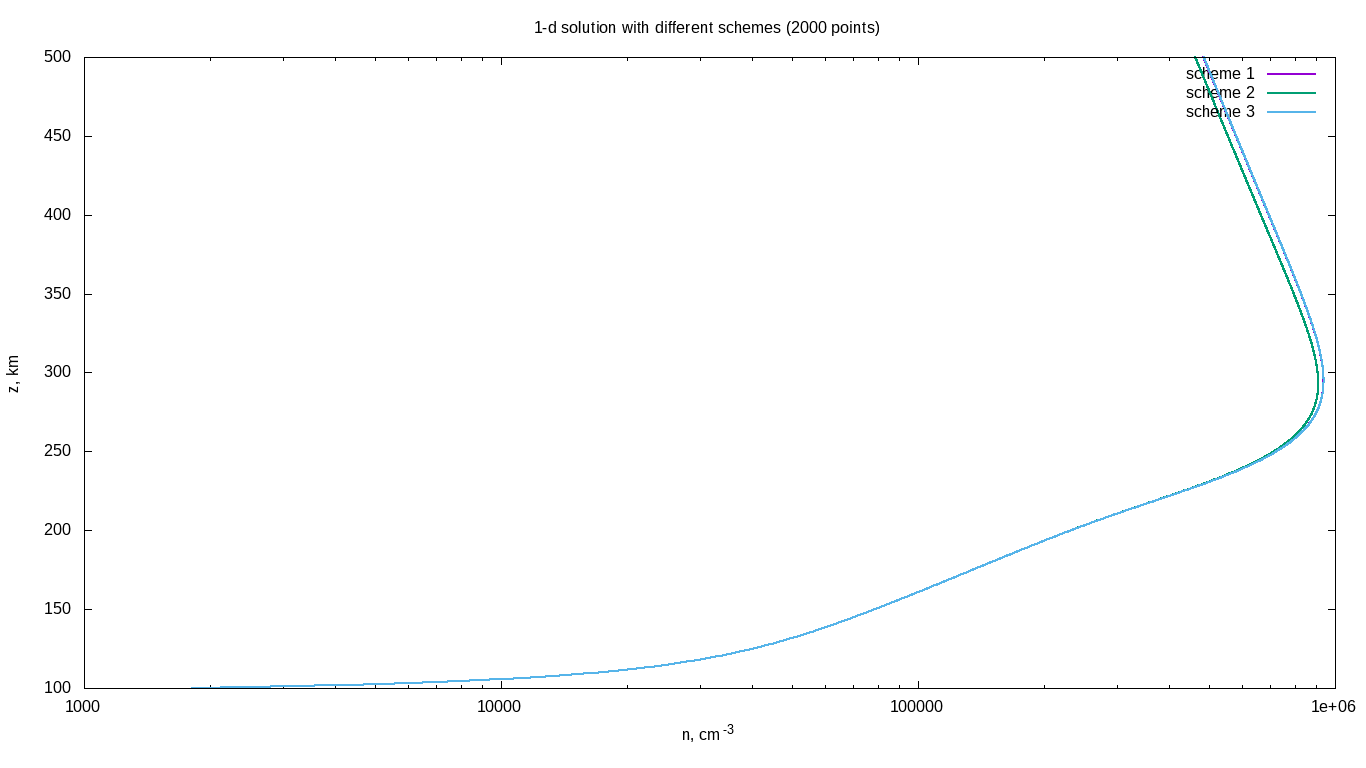
\includegraphics[scale=0.33]{1d_stationary_logscale_2000}}
\caption{Стационарные решения на $2000$ расчётных узлах.}
\end{figure}
\end{frame}


\subsection{Чувствительность к изменению внешних параметров}
\begin{frame}\frametitle{Чувствительность к изменению внешних параметров}

Варьирование входящих в уравнение температур показывает, что наибольшую чувствительность решение имеет к температуре нейтральных молекул.

\begin{figure}
\center{
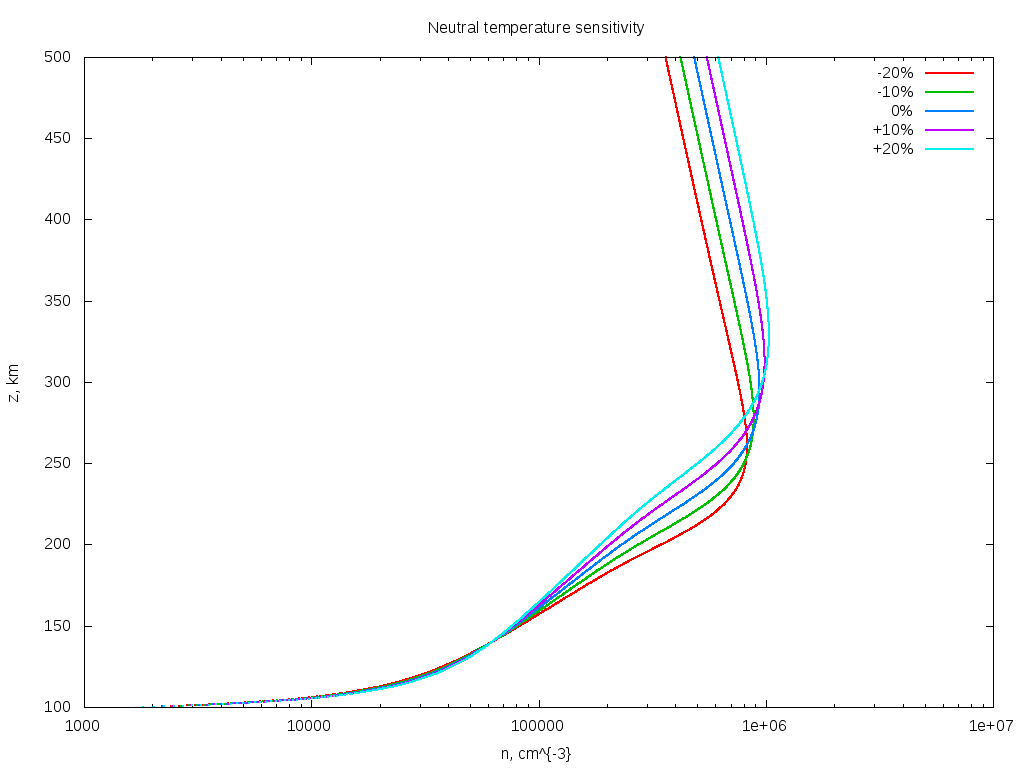
\includegraphics[scale=0.3]{Tn-sensitivity_log}}
\caption{Чувствительность к изменению температуры нейтральных молекул.}
\end{figure}

\end{frame}


\subsection{Учёт широтной зависимости}
\begin{frame}\frametitle{Учёт широтной зависимости}
Различные постановки используются для учёта наклонения магнитных силовых линий. 

Полученные стационарные решения при широтах $\varphi = -30^\circ$ и $\varphi=-2^\circ$:


\begin{figure}[H]
\begin{minipage}[c]{0.490\linewidth}
\flushleft
\center{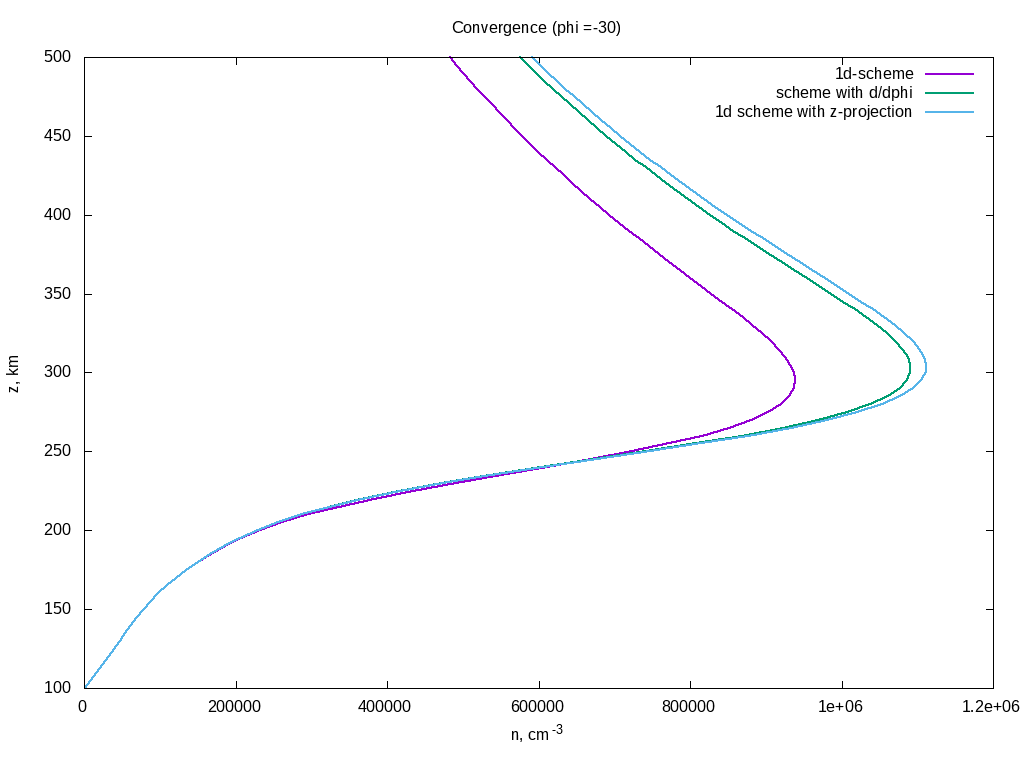
\includegraphics[scale=0.2]{stationary_-30}\\$\varphi = -30^\circ$.}
\end{minipage}
\hfill
\begin{minipage}[c]{0.490\linewidth}
\flushleft
\center{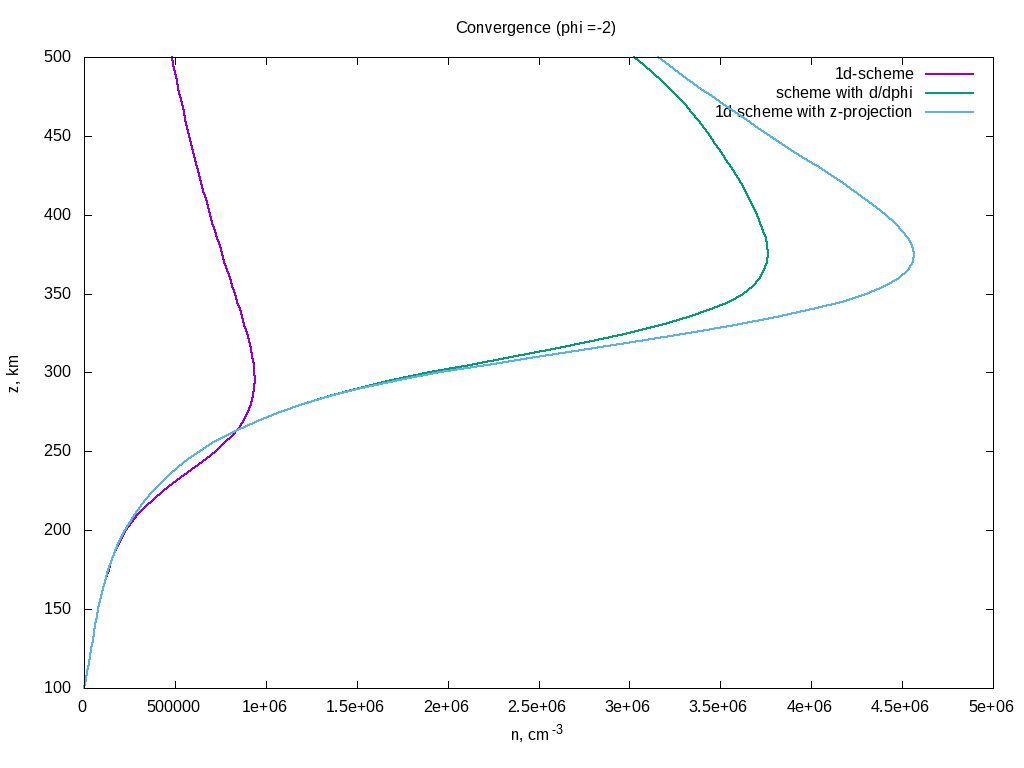
\includegraphics[scale=0.2]{stationary_-2}\\$\varphi = -2^\circ$.}
\end{minipage}
\end{figure}

\end{frame}


\subsection{Моделирование суточного хода}
\begin{frame}\frametitle{Моделирование суточного хода}

Вычисляется стационарное решение одномерной задачи при дневном значении $P(z)$, затем итерации по времени продолжаются с меняющимся $P(z, t)$.

\begin{figure}[H]
\center{
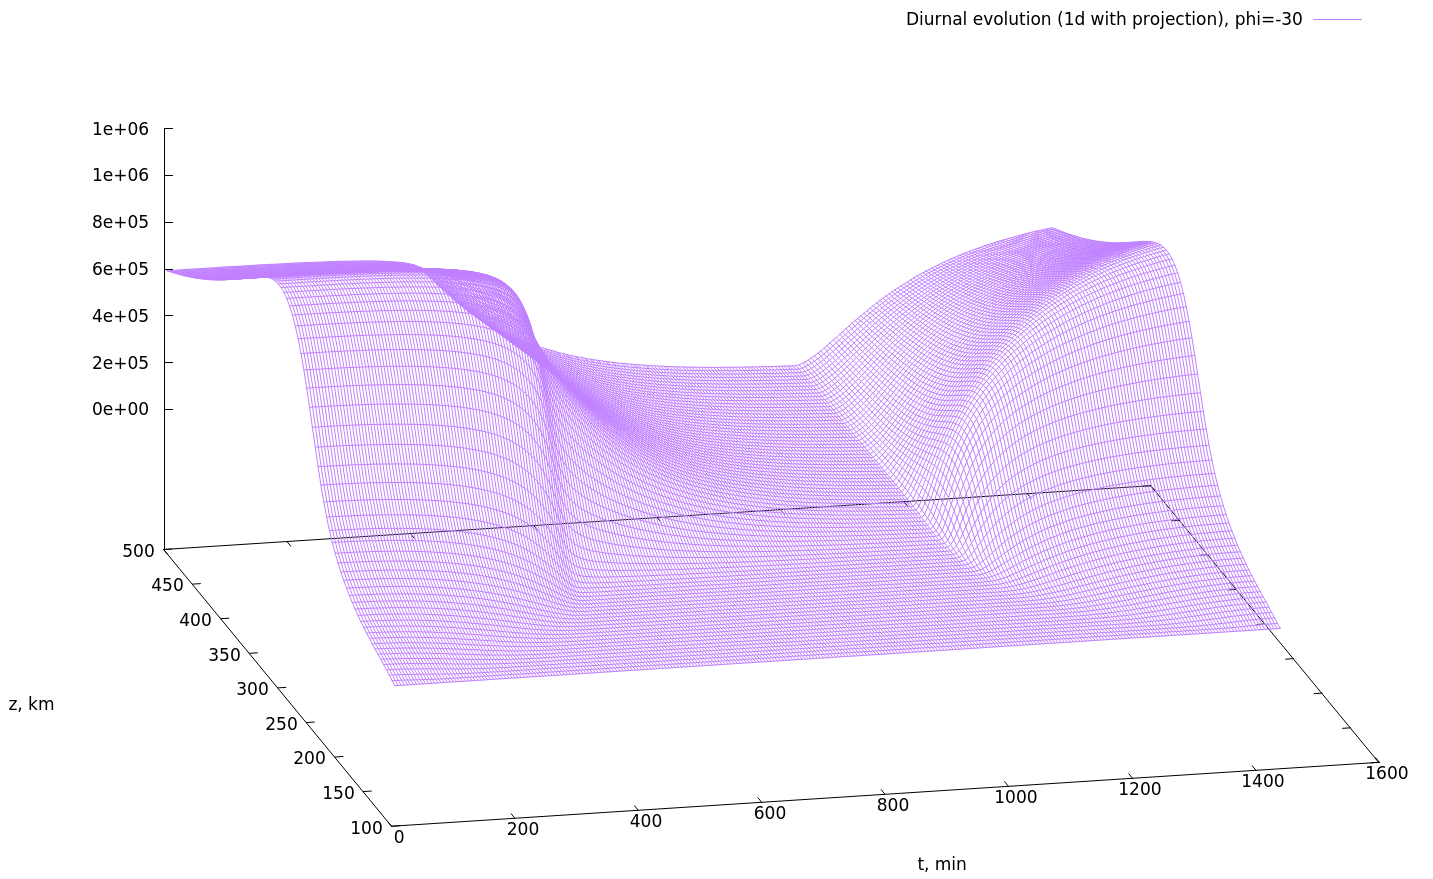
\includegraphics[scale=0.2]{diurnal_projection_-30}}
\caption{Суточный ход в одномерной модели с учётом проекции, $\varphi = -30^\circ$.}
\end{figure}

\end{frame}

\section{Список использованной литературы}
\begin{frame}\frametitle{Список использованной литературы}

\begin{itemize}
\item[1.] Kulyamin, D. V. and V. P. Dymnikov. A three-dimensional model of general thermospheric circulation. // Russian Journal of Numerical Analysis and Mathematical Modelling. 2013. 28(4): 353-380.
\item[2.] Кулямин Д.В., Дымников В.П., Моделирование климата нижней ионосферы. // Известия Российской академии наук. Физика атмосферы и океана, 2015. Т. 51(3): С. 317–337.
\item[3.] Schunk, R.W. and A.F. Nagy, IONOSPHERES Physics, Plasma Physics, and Chemistry. 2009, New York, United States: Cambridge University Press.
\end{itemize}

\end{frame}

\begin{frame}[plain]
  \begin{center}
  {\Huge Спасибо за внимание!}
  \end{center}
\end{frame}



\end{document}
